\paragraph{}
We want to explore the behavior of the used linear solver using domain decomposition methods for our inverse iteration algorithm.
We reming that we used GMRES and domain decomposition method RAS with 2 domains per process for the previous examples.
We compare the runtimes of solving 50 linear systems with different number of processors, for different solvers with and without preconditioner:

\begin{figure}[H]
 \centering
 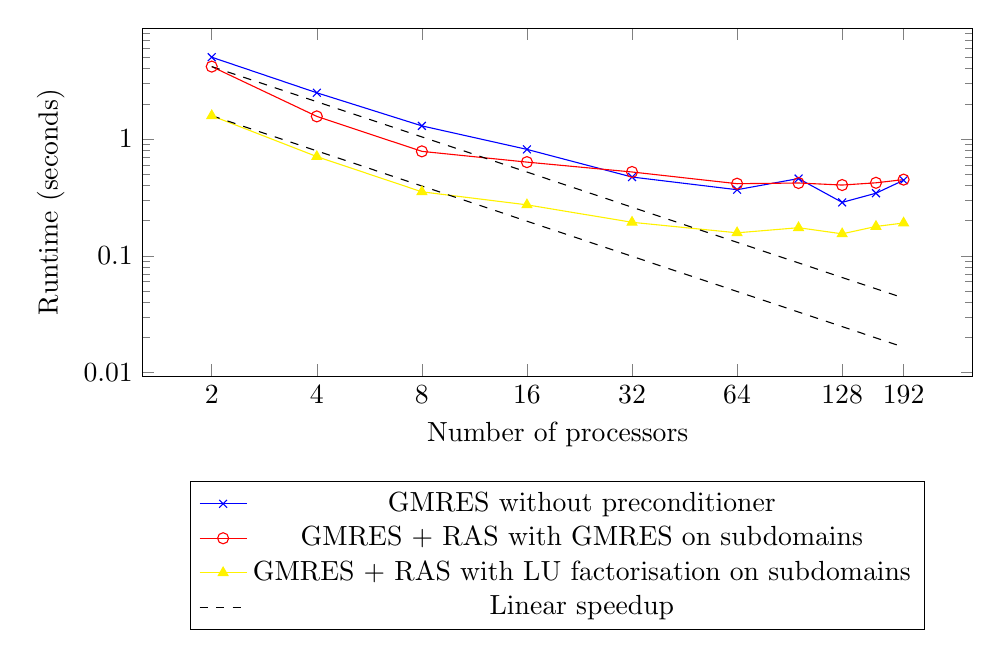
\begin{tikzpicture}
 \begin{axis}[
  height=6cm,
  width=\textwidth,
  xlabel=Number of processors,
  xtick={2, 4, 8, 16, 32, 64, 128, 192},
  xmode=log,
  ymode=log,
  log ticks with fixed point,
  ylabel=Runtime (seconds),
  legend style={
   at={(0.5, -0.3)},
   anchor=north
  }]
   \addplot[color=blue, mark=x] coordinates {
    (2, 5.019035956)
    (4, 2.489311578)
    (8, 1.295918689)
    (16, 0.8153684889)
    (32, 0.4725504889)
    (64, 0.3680468222)
    (96, 0.4586239333)
    (128, 0.2866520667)
    (160, 0.3435106444)
    (192, 0.4434605778)
   };
   \addlegendentry{GMRES without preconditioner}
   \addplot[color=red, mark=o] coordinates {
    (2, 4.171304311)
    (4, 1.562855289)
    (8, 0.78404696)
    (16, 0.6342229867)
    (32, 0.5220878222)
    (64, 0.4143123111)
    (96, 0.4201508889)
    (128, 0.4034540222)
    (160, 0.4217084444)
    (192, 0.4490838667)
   };
   \addlegendentry{GMRES + RAS with GMRES on subdomains}
   \addplot[color=yellow, mark=triangle*] coordinates {
    (2, 1.583247378)
    (4, 0.7071820222)
    (8, 0.3530209556)
    (16, 0.2730702667)
    (32, 0.193635)
    (64, 0.1572552667)
    (96, 0.1740185111)
    (128, 0.1541527111)
    (160, 0.1782941778)
    (192, 0.1908772667)
   };
   \addlegendentry{GMRES + RAS with LU factorisation on subdomains}
   \addplot[color=black, domain=2:192, dashed] expression {
    4.171304311*2/x};
   \addlegendentry{Linear speedup}
   \addplot[color=black, domain=2:192, dashed] expression {
    1.583247378*2/x};
 \end{axis}
\end{tikzpicture}

 \caption{Runtime of the linear solver with and without preconditioner.}
\end{figure}

We observe that using a domain decomposition method as preconditioner for our dense systems shows better runtime performances for both CG and GMRES.
The conjugate gradient method is applicable because the input matrix \(\Lapl_A\) is symmetric and so is the RAS preconditioner.
Solving the subdomains using a direct solver as the LU factorisation shows...
